%!TEX root = gutter+stars.tex
\chapter{Introduction}

Despite common belief, software engineers do not spend most time writing code. An approximate 50--90\% of development time is spend on code navigation and understanding \cite{Abra04a,Lato06a,Ko07a}. This may include reading of local source code and documentation, searching the internet for tutorials and code examples, but also seeking the help of other developers. User studies \cite{Lato06a,Ko07a,Sill06a,Frit10a,Kuhn10x} have found that software engineers use at least four kinds of cognitive clues for \codenavigation: 
	lexical clues, %\cite{a,b,c,d,e}, 
	social clues, %\cite{Lato06a,more}, 
	episodic clues %\cite{a,b,c} 
	and spatial clues. %\cite{a,b,c}. 

Examples of \codenavigation clues are 
	searching for an identifier name (lexical clue),
	contacting a coworker with known expertise (social clue), 
	referring to a design decision that was made years ago (episodic clue), or 
	scrolling to a piece of code by recalling its position within the source text file (episodic clue). 

Tool support for \codenavigation, however, is typically limited to keyword-based text file processing and hyperlinking of code elements. 

In our research, we are interested in how to support software engineers when they are facing technical questions that involve code navigation and code understanding. In interviews with professional software engineers, we investigated how developers find answers to technical questions in order to learn about their \codenavigation strategies. We found that the way towards an answer is typically split in two parts. In the 1)~first part, developers aim to turn their fuzzy initial clue into a more concerete textual clue, for example by running a series of web searches and inspecting the results. In the 2) second part, they use that newly found textual clue to query local documentation or resourced on the internet for the answer. We found that they particularly struggle with resolving social, episodic and spatial clues during the first part. This behavior might be an artifact of current tool limitations, that is developers aim to find a lexical clue first because other clues are harder to follow-up, or it might be a general search strategy. In either case, developers do need better tool support to follow-up non-lexical, \ie social, episodic and spatial clues.

Of the four kinds of clues that software developers use, spatial clues stand out for not having a first-class representation in the ecosystem of source code. Textual clues typically relate to identifiers found in source code or to terms used in comments and documentation. Social clues typically relate to coworker or experts from the personal network. Episodic clues relate to past experience which is often recorded in the version control system and in mailing list archives, at least partially. Spatial clues however typically lack such a first-class counterpart since software do not have an inherent spatial structure. Nevertheless, we found that developers do refer to \adhoc spatial properties, auch as the position of a piece of code on-screen or within a source text file. 

Given the potential of spatial clues for code navigation, we focused our research on how to support code navigation and understanding with spatial representations of software systems. A key contribution of this dissertation is thus \emph{Software Cartography}, a novel cartographic visualization of software systems that enables code orientation by on-screen spatial clues \cite{Kuhn08a,Kuhn10b}. Code maps, as we call them, are a stable and spatial representation of software systems based on lexical information found in the system's source code. Code maps are stable over time, and can be used by individual developers as well as shared by a team. We evaluated our approach in a qualitative user study, with both professional and student users, and found that it is most helpful for exploring search results and call hierarchies \cite{Kuhn10c}.

%%%%%%%%%% Section 1.1
%%%%%%%%%%
%%%%%%%%%%
%%%%%%%%%%
%%%%%%%%%%
%%%%%%%%%%

\section{Types of Code Navigation}

In the context of this work, we are interested in supporting software engineers when they are facing technical questions that involve a system's code base. We introduce the term \emph{\codenavigation{}} in order to refer to those navigation and understanding activities that happen while developer are looking for an answer to their technical question. Code orientation is thus am umbrella term for code navigation, software exploration and program comprehension. 

In the following we aim to characterize \codenavigation activities according to the kind of cognitive clues being followed-up (lexical clues, social clues, episodic clues and spatial clues) and characterize \navigation tasks according to their aim (refind, discovery and learning) and their reach (ranging from current working set to the entire internet). 

\subsection*{Aim and Reach of Code Orientation}
	
The aim of code orientation tasks can be one of the following three: a) refinding a given piece of code or functionality that you encountered or heard of in the past, b) discovering a piece of code that you know must exist by searching your local code repository or code examples on the internet, or c) learning how to implement a certain piece of code, by talking to people with expertise, by reading a book, or by finding advice on a mailing list or a blog post. 

The reach of code orientations can range from the current working set to the entire internet. The current working set can be a single method or all open files. The local codebase can be the current project and the entire codebase of a developer's company, but also includes all local documentation and learning resources. Eventually the ultimate reach is accessing the internet, which offers two kind of codebases. On the one hand there are dedicated code repositories that only contain source code, on the other hand, there is an amazing amount of code examples that are contained in blog posts and websites. The latter are a typically more useful for code orientation since they are collaboratively pre-filtered, \ie the authors of the embedding content carefully selected those examples for their usefulness for learning and copy-pasting. 

When moving from a local to a global reach, the nature of information resources changes. Local information sources are typically limited, homogenous and authored by a small group of trusted people with known expertise. More global information sources are typically unlimited, heterogenous and authored by people with unknown expertise and unknown trustworthiness.

The reach of  code orientation is often given by its reach. For example, refinding tasks are typically targeted at the local codebase, with which the developers are familiar, whereas discovery and learning tasks are typically targeted at the internet. But just as likely, parts of the local code based might be unknown to a developers and thus become target of a discovery task, or it may be that a developer recalls to have read about the solution on the internet and attempts to refind information at a global scale on the internet.

In the following, we enumerate code orientation clues by category. We motivate their use by developers, provide examples, shed light on underlying assumptions, and discuss current tool support and its shortcomings.

\subsection*{Orientation by Lexical Clues}

% Importance
Lexical clues are by far the most common clue used by software engineers for \codenavigation. 
% Examples
Examples of lexical clues are recalling the name of an identifier or algorithm, or having a guess about a keyword used by others in order to search the web for documentation or code examples. 

% Assumption
Developers do rely on lexical clues because they assume that names are meaningful, that there is a meaning to names and that names have been meaningfully chosen. 
% Kind of information?
Lexical clues are typically pointers to lexical information that is present as identifier names or in comments. However, lexical information is not limited to source code but also found in the content of emails, bug reports and web pages. For example, following-up a lexical clue might guide the developer to a wikipedia page that contains the algorithm he's looking for. 

% Tool support and hint a need that we address later on?
Simple keyword search and regular expressions are of great help to follow-up on a lexical clue. However, a major problem with lexical clues is that developers have to make a guess about how other people name things. Using information retrieval and natural language processing can help to go beyond the limitation of development tools that are based on exact keyword matches. 

\subsection*{Orientation by Social Clues}

% Importance
Social clues are often not considered part of software comprehension, yet they are most helpful for discovery and learning. User studies have shown that coworkers are the most frequent source of information after the source code itself and in particular more frequently turned to than documentation \cite{Ko07a}.
% Examples
Examples of social clues can be asking coworkers or experts from the personal network for help, or posting a question to a discussion board on the web where international experts share their expertise. 

% Assumption 
Developers do rely on social clues because they assume that people do have expertise, in particular that other people do have more or different expertise so they can be of help to find answers. The knowledge in the mind of team members is typically more accurate than documentation. 
% Kind of information?
Social clues are typically pointers to other persons from the developer's personal network, either a co-worker or a friend. However, social clues are not limited to the personal network but can also be pointers to mailing lists and other expert groups that are ready to share their expertise online on the internet.

% Tool support and hint a need that we address later on?
Support for code orientation by social clues is typically not present in development tools, thus the current state of the art is that developer have to recall the name of a person with expertise. This basically boils down to a lexical clue that has to be used a proxy for the actual social clue that developer does want to follow-up. Using techniques and ideas drawn from social media can help to go beyond the limitation of a developer's personal network.

\subsection*{Orientation by Episodic Clues}

% Importance
Episodic clues are most helpful to refind source code that has been written or used in the past, since as humans we have strong episodic memories. 
% Examples
Episodic clues are typically tied to personal memory, as for example in recalling the first-hand experience of a conference talk or of a pair programming session. 

% Assumption 
Developers do rely on episodic clues because they assume that their knowledge in the past has been more accurate than their current knowledge. Which is a valid assumption because as humans our episodic memory works way better than our structural memory, typically developers do recall ``that'' they knew the answer before but not ``what'' the answer exactly constituted of.  

% Kind of information?
Episodic clues are typically pointers to past interaction with books, mailing lists and other people, but may also be pointers to past snapshots of the current or a related software system. 
% Tool support and hint a need that we address later on?
Support for code orientation by episodic clues in development tools is typically not present. Information related to episodic clues is often stored in external databases, such as version control repositories and mailing list archives, and thus not integrated with development tools. Using data mining techniques and embedding the results in a story-telling visualizations can help to go beyond the limitation a single developer's personal experience with a system's history.

%- or you know ''we had this bug a year ago'' or you know ''oh we need to sort a list, we've done this in this project'' ... episodic memory ... or you recall who've told you about it ... 
%- Episodic memory ... recall that they've solved it ... or that they've seen the solution on a mailing list ... learning by lurking ... grown your own folksonomy ... collect your own anecdotes
%- Chronia: ownership map shows how contributers to a software system worked together ... devs get excited ... ''see here we worked together'' .. even better than a holiday photo album.

\subsection*{Orientation by Spatial Clues}

% Importance
Spatial clues may help to reduce the cognitive load of a user's orientation in a hyperlinked document space, such as software systems. 
% Examples
% Kind of information?
Spatial clues can be of three kinds, either they are structural or conceptual as in recalling which class or architectural layer some functionality belongs to, or they are true spatial clues as in recalling the on-screen or within-text-file position of a given function.

% Assumption 
Developers do rely on spatial clues because as humans they have strong spatial capabilities. The spatial capabilities of our brain are impressive: it has been found that developers do form a spatially meaningful internal mental model of software systems even though the external representation of source code has no inherent spatial properties by itself. 

% Tool support and hint a need that we address later on?
Current support for code orientation by spatial clues in development tools is \adhoc at best. The systems is presented as a tree view of alphabetically ordered files and inside a file the source is linearized as an unordered text file. While this might accidentally help to refind some code by a spatial clue, support for the discovery of yet unknown source code by spatial clues is limited to structural clues. Providing developers with a cartographic visualization, so they can use spatial on-screen clues for navigation and understanding of code, may help to go beyond the limitation of software's missing spatial structure.

%%%%%%%%%% Section 1.2
%%%%%%%%%%
%%%%%%%%%%
%%%%%%%%%%
%%%%%%%%%%
%%%%%%%%%%

\section{Thesis Statement}

We state our thesis as follows

\begin{quote}
To support software engineers when they are facing technical questions, 
that involve a system's source code, 
we need development tools that tap on unconventional information found 
in source code in order to provide developers with code orientation clues 
that would be out of their reach without tool support.
%better tool support for social clues and episodic clues. And third, since software has no inherent spatial dimensions, we need to establish a stable cartographic representation of software systems based on other properties in order to facilitate code orientation by on-screen spatial clues.
\end{quote}

%%%%%%%%%% Section 1.3
%%%%%%%%%%
%%%%%%%%%%
%%%%%%%%%%
%%%%%%%%%%
%%%%%%%%%%

\section{Contributions}

In this work, we present the following contributions that explore the support of code orientation clues by development tools. Common to all these contributions is that they tap on unconventional information found in source code in order to provide developers with code orientation clues 
that would otherwise be out of their reach. For example, in \autoref{the chapter on chronia} we present a story-telling visualization of a system's history that enables new hires to draw on episodic memories that they would not have access to otherwise.

Each of these contributions has been published as one or more peer-reviewed publications at international conferences or in international journals. 

%%%%%%%%%%
\subsection*{Software Cartography}
\infobox
	{Code orientation in general}
	{Local codebase and possibly history of a system}
	{Spatial (established through lexical and structural information)}
	{Visual analytics of a cartographic visualization}

Current tool support for code orientation by spatial clues is \adhoc at best, most striking is the lack of spatial on-screen representations of source code. Without such a representation, developer are barely able to draw on the strong spatial capability of the human brain. 

We provide a cartographic on-screen visualization so they can start using spatial clues for code orientation. Since software has no inherent spatial structure, we use lexical and structural information found in the source code to establish a spatial layout of the local code base. Code maps, as we call them, are stable over time and can be shared among members of a team to establish a common mental model of the system. 
%
We implemented our approach in a prototype, evaluated it in a user study, and found that it is most helpful for spatially exploring search results and call hierarchies.

For more information please refer to the next section for a brief introduction, and to \autoref{the chapter on codemap} and \autoref{the chapter on the codemap user study} for an in depth coverage. 

The work on software cartography has been realized with the support of my students David Erni and Peter Loretan, and has been published as two peer-reviewed conference paper \cite{Kuhn08b,Kuhn10c}, one of which has been extended into a peer-reviewed journal paper \cite{Kuhn10b}, as well as their Master's theses \cite{Erni10a,Lore11a}. 

%%%%%%%%%%
\subsection*{Lexical Clustering}
\infobox
	{Refinding and discovering topics}
	{Local codebase of a system}
	{Lexcial (established through lexical information)}
	{Visual analytics and fuzzy keyword search}

Keyword matching and regular expressions are powerful means for code orientation by lexical clues. However, current tool support fails to meet the developer needs when they are following-up on a fuzzy lexical clue. 

We present an approach to model a system lexical information in a fuzzy text model that resolves synonymy and polysemy with unsupervised learning. We use the fuzzy text model to cluster the parts of a system by topic, and visualize the topics using correlation matrices and \emph{distribution maps}, a novel visualization that illustrates the distribution of topics over the packaging of a system. 
%
We implemented the approach in a prototype and evaluated its application.

For more in information please refer to the \autoref{the chapter on lexical clues}. 
%
The work on lexical clustering (formerly also known as ``semantic clustering'') has been published a peer-reviewed conference paper \cite{Kuhn05a} which has been extended into my Master's thesis \cite{Kuhn06a} and into a peer-review journal paper \cite{Kuhn07a}.

%%%%%%%%%%
\subsection*{Code Summarization}
\infobox
	{Refinding and discovering topics}
	{Part of a system's codebase or history}
	{Lexcial and episodic (established through lexical information)}
	{Visual analytics of word clouds}

When developers encounter a piece of source code for the first time, they are typically not presented with a high-level summary of the code's topics. We present an approach to summarize part of a system as a word cloud, that consist of the statistically most significant terms that set this part of system apart from the rest. The same approach can be use to compare two parts of the same system or to compare two versions of the same system. Presenting those word clouds to the developer helps them to lexically query the topics, as well as when presenting all words clouds of a systems versions to recover and tell the story of a systems history and thus enabling developers to draw from episodic memories that they possibly never experienced first-hand.
%
We implemented the approach in a prototype and evaluated its application.

For more in information please refer to the \autoref{the chapter on LogLR}. 
%
The work on code summarization has been published as a peer-reviewed conference paper \cite{Kuhn09a}.

%%%%%%%%%%
\subsection*{Stories of Collaboration}
\infobox
	{Learning about team collaboration}
	{Team of a project's local codebase}
	{Episodic (established through social and historical information)}
	{Visual analytics of a story-telling visualization}

Episodic clues are of great help to developers when having to find their way through a system, however episodic memory is only available to those developer that know the system's history first-hand. We present an approach to recover and tell a systems history as a story-telling visualization. Our approach uses social and historical information taken from the version control system to establish an episodic visualization of the system's history. Both new hires and seasoned team members can use this visualization to learn about episodes from the system's history in order to take better technical decisions when working with the system in the future.
%
We implemented the approach in a prototype and evaluated its application.

For more in information please refer to the \autoref{the chapter on LogLR}. 
%
The work on visualizing code ownership is part of Mauricio Seeberger's Master's thesis \cite{Seeb06a} and has been published as a peer-reviewed conference paper \cite{Girb05a} that was co-authored by our mutual supervisor Tudor G\^irba and myself.

- Understanding who owns a piece of code 50\% \cite{Latoza} 

%%%%%%%%%%
\subsection*{Discovery of Experts}
\infobox
	{Discovery of experts}
	{Experts that committed to local codebase}
	{Social (established through lexical and historical information)}
	{Fuzzy problem description given as natural language text}

Given current tool support, following up social clues has to be done through the lexical proxy of a person's name. We present an approach to discover experts without having to know their name. Given a problem description, such as a work item or a bug report, we provide an automated means of linking to the person with the expertise on that matter. We use lexical information found in the submission to the version control system in order to model the developer's expertise. 
%
We implemented the approach in a prototype and evaluated it against a benchmark in bug-report assignment .

The work on discovery of experts has been realized by my student Dominique Matter, and has been published as a peer-reviewed conference paper \cite{Matt09a} that he first-authored as well as his Master's thesis \cite{Matt09b}.

%%%%%%%%%%
\subsection*{Credibility of Code Search}
\infobox
	{Discovery of trustworthy projects}
	{Open-source projects on the internet}
	{Episodic (established through social and historical information)}
	{Name of an open-source project}

Searching for code examples or libraries on the internet is a common code orientation task. In interviews with developers, we have found that credibility is one of the major issues when copying source code from an external and thus untrusted source such as the internet. We present an approach to automatically asses the trustworthiness of open-source projects based on the credibility of their authors, in inferring the trustworthiness of well-known project to unknown projects if they have common contributors. 
%
We implemented the approach in a prototype and evaluated it against a benchmark in bug-report assignment .

The work on discovery of experts has been realized by my student Florian Gysin, and has been published as a peer-reviewed workshop paper \cite{Gysi10b} that he first-authored as well as his Bachelor's thesis \cite{Gysi10c}, in addition his work won the ACM Student Competition award 2010 \cite{Gysi10a}.

%%%%%%%%%% Section 1.4
%%%%%%%%%%
%%%%%%%%%%
%%%%%%%%%%
%%%%%%%%%%
%%%%%%%%%%

\section{Software Cartography in a Nutshell}

Current tool support for code orientation by spatial clues is \adhoc at best, most striking is the lack of spatial on-screen representations of source code. Without such a representation, developer are barely able to draw on the strong spatial capability of the human brain. With \SOCA we aim to address this limitation. We provide a cartographic on-screen visualization so that software engineers can start using spatial clues for code orientation. Since software has no inherent spatial structure, we use lexical and structural information found in the source code to establish a spatial layout. 

\SOCA embeds a cartographic visualization of the current working set in the development environment (IDE) of software engineers. Code maps, as we call them, are stable over time and can be shared among members of a team to establish a common mental model of the system. Code maps are most useful when they supports as many development tasks as possible with spatial clues. Therefore we integrated \SOCA in the IDE so that a map of the software system may always be present and may thus support as many development tasks as possible. 

At the moment, the \Codemap prototype plug-in for \eclipse supports the following development tasks:\footnote{New features are added on a weekly base, please subscribe to \url{http://twitter.com/codemap} to receive latest news.}

\begin{itemize}
\item Navigation within a software system, be it for development or analysis. \Codemap is integrated with the package explorer and editor of \eclipse. The selection in the package explorer and the selection on the map are linked. Open files are marked with an icon on the map. Double clicking on the map opens the closest file in the editor. When using heat map mode, recently visited classes are highlighted on the map.

\item Comparing software metrics to each other, \eg to compre bug density with code coverage. \Codemap is hooked into several \eclipse plug-ins in order to display their results on the map alongside the regular views. The map displays search results, compiler errors, and (given the \textsc{Eclemma} plug-in is installed) test coverage information. More information can be added through an extension point.

\item Social awareness of collaboration in the development team. \Codemap can connect two or more \eclipse instances to show open files of other developers. Colored icons are used to show the currently open files of all developers. Icons are colored by user and updated in real time.

\item Help to understand a software system's domain. The layout of \Codemap is based on structure \emph{and} vocabulary, since we believe that a mental model of software should transcend structural artifacts. Labels on the map are not limited to class names, but include automatically retrieved keywords and topics.

\item Exploring a system during reverse engineering. \Codemap is integrated with \eclipse's structural navigation functions such as search for callers, implementers, and references. Arrows are shown for search results. We apply the \textsc{Flow Map} algorithm \cite{Phan05a} to  avoid visual clutter by merging parallel arrow edges. \autoref{fig:awesome} shows the result of searching for calls to the {\tt \#getSettingOrDefault} method in the {\tt MenuAction} class .
\end{itemize}

\begin{figure}
\begin{center}
  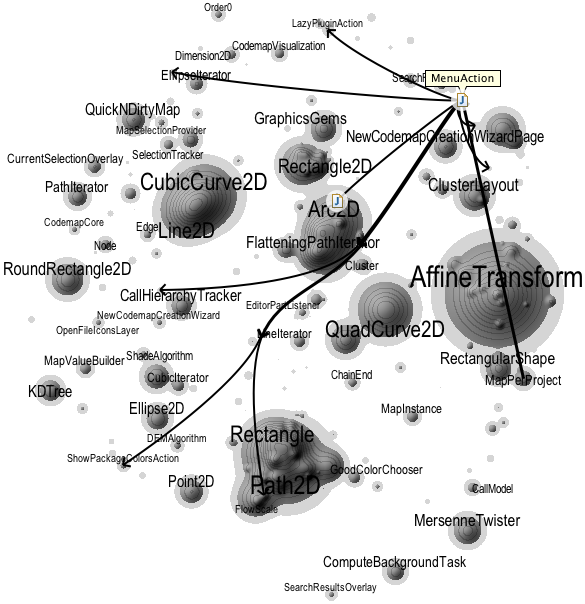
\includegraphics[width=0.75\linewidth]{fig/intro-codemap-example}
\end{center}
    \caption{\emph{Thematic codemap of a software system, here the \Codemap tool itself is shown. Arrow edges show outgoing calls from the {\tt \#getSettingOrDefault} method in the {\tt MenuAction} class, which is currently active in the editor and thus marked with a speech-balloon label.}}
    \label{fig:awesome}
\end{figure}

\begin{figure*}
\begin{center}
  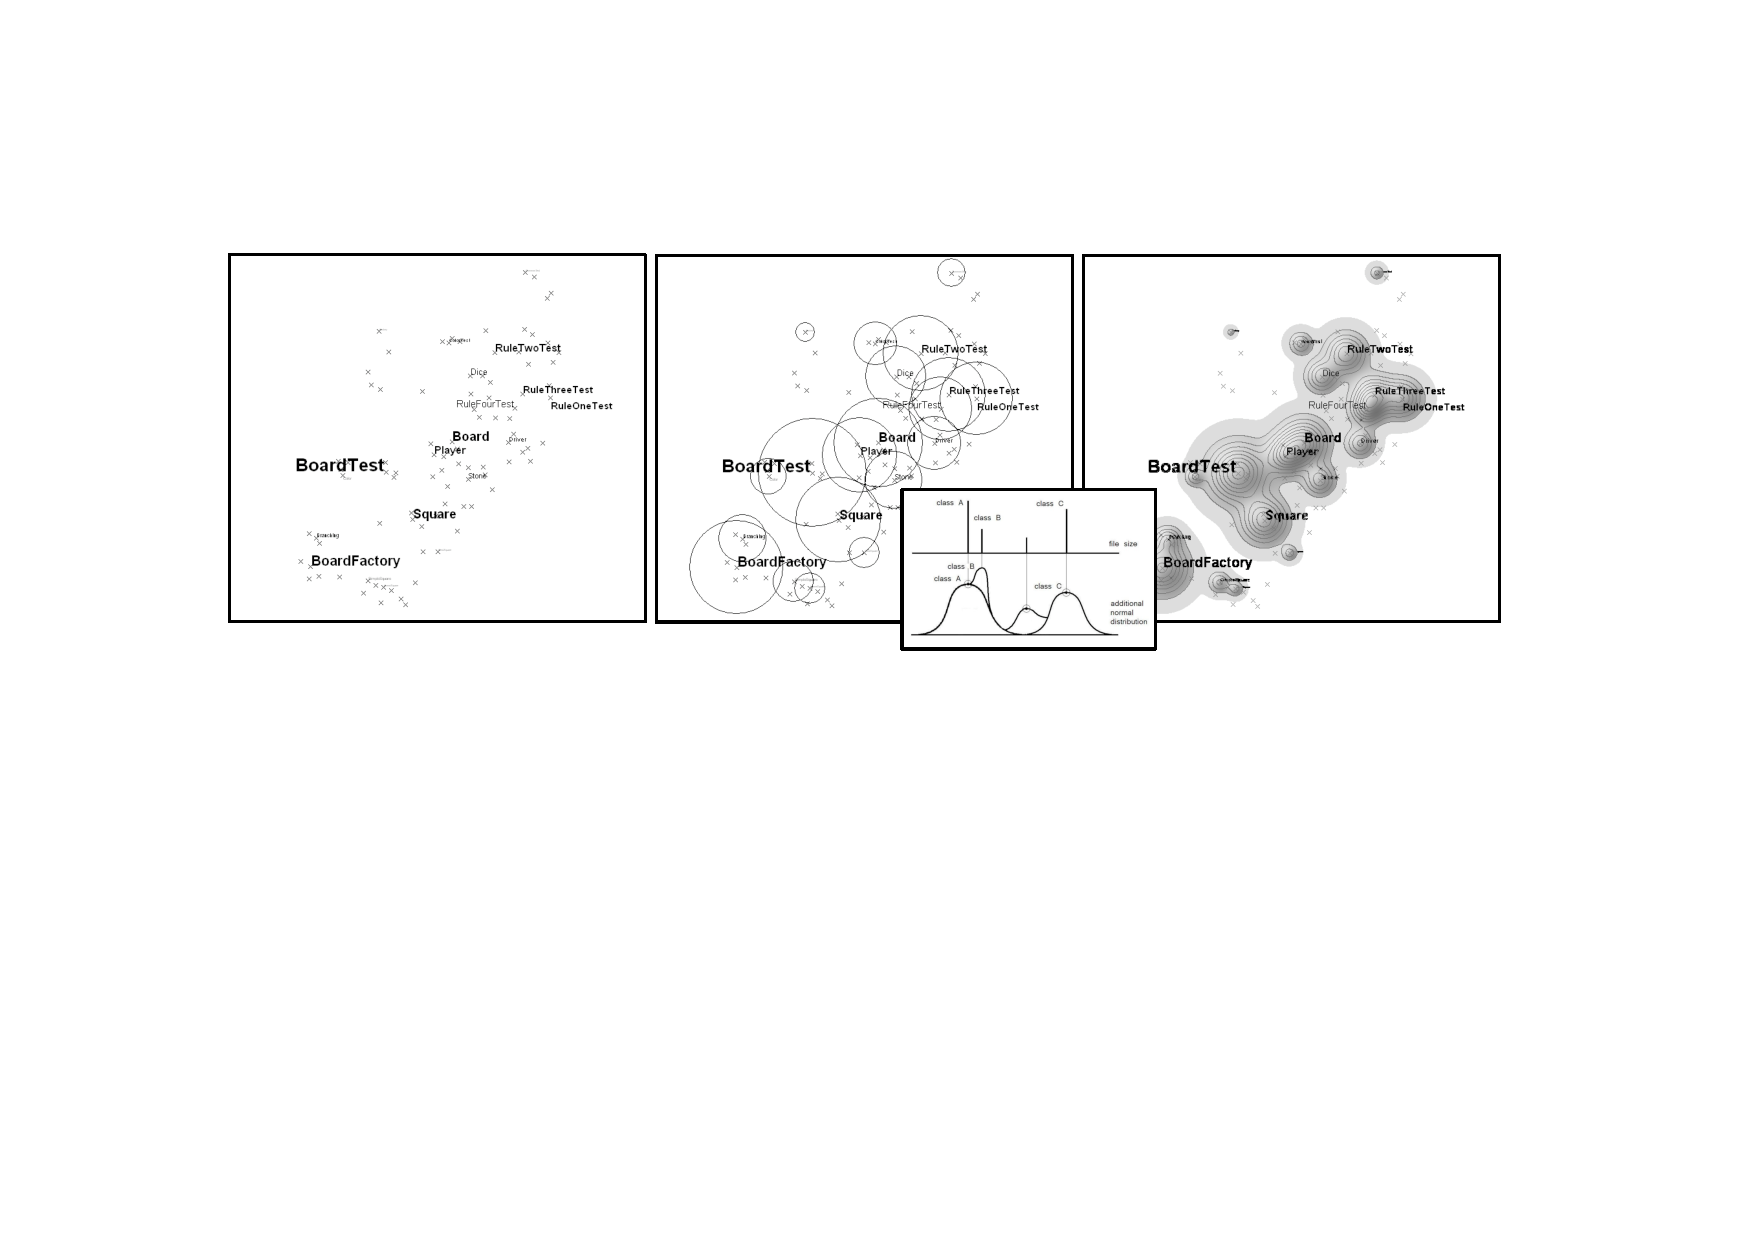
\includegraphics[width=\linewidth]{fig/intro-pipeline}
\end{center}
    \caption{\emph{Construction steps of a software map, from left to right: 1) 2-dimensional embedding of files on the visualization pane; 2.a) circles around each file's location, based on class size in KLOC; 2.b) each file contributes a Gaussian shaped basis function to the elevation model according to its KLOC size; the contributions of all files are summed up; 3) fully rendered map with hill-shading, contour lines, and filename labels.}}
    \label{fig:steps}
\end{figure*}

\subsection*{Construction of a Code Map}

\autoref{fig:steps} illustrates the construction of code maps. The sequence of the construction is as follows:

\begin{description}

\item[2-Dimensional Embedding]
A metric distance is used to compute the pair-wise dissimilarity of software artifacts (typically source code files). A combination of the Isomap algorithm \cite{Tene00a} and Multidimensional Scaling \cite{Borg05a} is used to embed all software artifacts on the visualization pane. Different to lexical clustering Latent Semantic Indexing is not anymore; it has been found to have little impact on the final embedding, if at all. The application of Isomap is an improvement of the embedding in order to assist MDS with the global layout. The final embedding minimizes the error between the dissimilarity values and the visual distances.

Early prototypes of \Codemap used a distance metric that was based on lexical similarity only. However, our user study revealed that developers tend to interpret visual distance as a measure of structural dependencies, even though they were aware of the underlying lexical implementation. Based on this observation, we developed an improved distance metric that takes both lexical similarity and structural distance (based on the ``Law of Demeter'' \cite{Lieb88a}) into account. 

\item[Digital Elevation Model] In the next step, a digital elevation model is created. Each software artifact contributes a Gaussian shaped basis function to the elevation model according to its KLOC size. The contributions of all software artifacts are summed up and normalized. 

Using KLOC leads to an elevation model where large classes dominate the codemap. Observations from our user study indicate that this might be misleading since developers tend to interpret size as a measure of impact. Based on this observation, we implemented a set of different impact metrics~\cite{Lanz06a} and plan to evaluate them in a fresh user study.

\item[Cartographic rendering] In the final step, hill-shading is used to render the landscape of the software map. Please refer to previous work for full details~\cite{Kuhn08b}. Metrics and markers are rendered in transparent layers on top of the landscape. Users can toggle separate layer on/off and thus customize the codemap display to their needs.

\end{description}

%%%%%%%%%% Section 1.5
%%%%%%%%%%
%%%%%%%%%%
%%%%%%%%%%
%%%%%%%%%%
%%%%%%%%%%

\section{Outline}

The dissertation is structured as follows

\begin{description}
% --> related.tex
\item[\autoref{the chapter on related work}] discusses related work. We present various user studies and solutions to code orientation and analyse the short comings in the context of each orientation clue.
% --> codemap.tex
\item[\autoref{the chapter on codemap}] introduces \emph{Software Cartography} as approach to establish a cartographic visualization that facilitates spatial code orientation by individuals or teams. The approach is implemented in the \textsc{Codemap} tool.
\item[\autoref{the chapter on the codemap user study}] reports on a qualitative user study that evaluates the prototype implementation of the Software Cartography approach presented above.
\item[\autoref{the chapter on the MSR user study}] presents a user study that looks at how developers find answers to technical questions and discusses code orientation by cognitive clues.
% --> gutter+stars.tex
\item[\autoref{the chapter on lexical clues}] presents an approach for clustering and summarizing of software systems using lexical information found in source code. The approach is implemented in the \textsc{Hapax} tool. 
\item[\autoref{the chapter on LogLR}] presents an approach that uses lexical information found in source code to summarize parts of a system, the whole system, or even the system's entire evolution. The approach is implemented in the \textsc{EvoClouds} tool.
\item[\autoref{the chapter on chronia}] presents an approach for addressing the episodic memory of developers by providing them with a visualization that tells the story of the team collaboration as recorded by the version control system. The approach is implemented in the \textsc{Chronia} tool.
\item[\autoref{the chapter on bug reports}] presents an approach that use lexical information found in contributions that developers shared with open source systems to build a recommendation model for bug repots. The approach is implemented  in the \textsc{Devlect} tool.
\item[\autoref{the chapter on codesearch}] presents an approach that uses cross-project collaboration of developers in open source projects to estimate the credibility of code search results. The approach is implemented in the \textsc{Bender} tool.
\item[\autoref{the conclusion}] concludes the dissertation and outlines future work.
\end{description}


%%%%%%%%%%%%

%Also there is a difference in finding code and finding functionality, like if a developer has never seen some piece of source code it is maybe easier to recall the person that has told him about it rather than recalling the source code's name. And just the same with the forward reaching tasks, where often copy-pasting an example is preferred over learning for pragmatic cost considerations.

%- Maybe you recall the song that played on the webradio, so you look that up ...
%- You can use one kind of information as a proxy for other information, so you can you use social and temporal information as a proxy for dependency information (like Tom Zimmermanns work on recommending other locations to update).
%- Photographic memory.
%- The clues have to be turned into actions.
%- How many (inter)actions do you have to do to follow up one clue.
%- Non-conventional questions that people ask themselves but had no tool to answer them before.
%- Two hard problems in CS, caching and naming.

%- JExample generates 'Examples that are worth to be found' .. JExample makes exampels more relevant and more applicable ...
%- Erwann: information can come right from the source code (lexical clues) and can come from somebody else (social clues) from temporal memory or version control system (temporal ones) ...
%- Clues are not about the sources of information, but about the way developers navigate about how they cognitively work when they follow.

%- Change on database propagates to business layer, UI layer ... you know where do go spatially, the space is given by space of software, in other case the space is given by layout of IDE, or given by storage format or persistence format, you know it is there in that text file or on that folder, or in smalltalk open in that window.
%- Codemap: if you observe which clues devs use to refer to code, you'll find all four, but if you look at tool support, you find lexical supported by tools, and temporal only in external tools, and social clues are also not supported, you gonna recall the name of person (ie using the lexical clue of the name as a proxy for the social connection) and spatial is not supported at all, we got the IDE layouted without care about spatial thinking ... code bubbles, code map, and code canvas are about the first systems to take care of this ... 
%- If you ask people to draw maps of their software systems ... as Grady Booch does ... and they always draw an architecture with spatial structural ... so the spatial structure is in their thinking but not in the IDE and even not in the software ...
%- So this why codemap is so interesting because it takes the lexical information and give it a spatial structure in the hope to fill the gap when devs are stuck with lexical clues or social/temporal
%- Spatial clues "somewhere at the end of this file"
%- Structural and spatial is often perceived in the same way, developers tend to use spatial terminology to refer to layers and architectural components.
% - To create a space of software that is visualized on screen, so that people can start using that one to navigate in source code.
%- Erwann: the mental model part?
%- To provide them with a space that will become / should reflect their spatial model...
%- Erwann: if the notion of mental model can be used for all clues ... the other tools gravitate around this spatial mental model.
	
%- All these tools help you to follow up, some more complex clues and unconventional information. It is not that any of these tools addresses a very specific task? Erwann thinks yes it does.
%- I want to help developers, working with code, in particular wrt navigation and understanding, and learning about code.  These clues can be  (ii)  or (iii) it could be temporal or episodic, having a memory from the past that could lead you to an answer, that you've seen it last year (or recall the song that played on the radio) or (iv) 
%- maybe in some years we can add here location based clues, like I've written that code on the train. And in the source of JUnit Kent Beck found it so cool that he added "was written on H�tte at 1200 mUm"
%- and sometime people follow up some very underdeveloped spatial clues. So we know they follow up these clues so we need better tool support and not have to be force to use lexical proxies, you should not be forced to recall the name, but be able to directly work social information when following up a social clues.
%- With spatial information we have this even more special situation that we possible first have to create a space for space.
%- Is there one space to rule them all? or different spaces for different tasks. Codemap that provides one space but still have IDE so onscreen is split, Codecanvas does the same but put the source code on it such that the space become the only onscreen space, the space should be contextually created.
%- The thesis emerged from my work, is that in order to support developers with code navigation we need to build better tools that address the cognitive clues that are used by developers, in particular (in addition to lexical clues) to support navigation by social clues by temporal clues and by spatial clues, and since software has no ...
%- lexical clues are present as identifier names and in comments, social clues are also there we know how has written software and mailinglists etc so people are also there as entity, and also temporal information is tere we have versioning systems that make snapshots of a system in time, but spatial is more difficult ...
%- it somehow maps to the structure of software, which you can extract from source code, but very often spatial is more on a conceptual level and people even use spatial terms on the very level of the arrangement of the UI on screen. So we have three spatial dimensions, structural, conceptual and on screen. So the spatial clues have the least support, so we gotta create a space of software of onscreen to support spatial navigation by developers. 
%- Since software lacks we need to create a spatial view to address the on-screen spatial clues. To create a cartographic representation of other non-spatial properties of the system (like temporal, social and lexical ones) and give them a spatial representation os people can use this forth kind of navigation clues that are actually used. When you talk with developers how they find answers to technical questions related to source code they will tell you sometime they recall a method is at the end of this file, which is onscreen spatial representation. Lemme browser the packages it us up there, down there. And they will use this in the same sentence as some spatial representation that is related to package structure. We have to fix this also up there in the business layer, it as down there in this file, we have to fix this up there it is down there in this file. 
%- Information retrieval to make more interesting things with lexical clues.
%- Evoclouds combine lexical with temporal information.
%- Work by Dominique Matter where we go and mine all the date from the temporal repository and mine the the vocabulary from the contribution of the developers, so we have a new tool that models the expertise of the developers so that now when you have a bug report the system can recommend to you the person. You can turn now a fuzzy textual clue into a social thing.
%- So we asses the credibility of search results solely based on the social network of the authors. This is the way developers have been found to asses the trustworthiness of code, since when you copy code from the internet you do so because you do not want to make the effort of technically understanding it so you look at its author's credibility to make an assessment of trustworthiness.
%- So we have the Chronia tool that has a timeline of the project, and you have a timeline of each file and you see the collaboration patterns. When you show this to developers the go crazy, with this visualization the episodic memory is brought back. You can learn about team members.


